\begin{frame}
	\frametitle{Focus: Theoretical Uncertainties}
	\vspace{10pt}
	{\scriptsize \href{https://indico.cern.ch/event/507870/contributions/1186978/attachments/1247701/1838325/pdf_uncertainty_treatment.pdf}{{\color{ATLASBlue}``Theoretical Uncertainties in Searches for Heavy Gauge Bosons at the LHC"}} - IOP 2016}\\
	
	{\scriptsize \href{https://indico.cern.ch/event/605722/contributions/2581151/attachments/1455384/2245967/PDFforum_10.03.2017.pdf}{{\color{ATLASBlue}``NNLO	QCD	PDF	Uncertainties for Drell-Yan	Production at 13 TeV"}} - Exotics/SUSY workshop 2017 (Bucharest) \& PDF forum }
	
	\vspace{-5pt}
	\li{Uncertainty of the parton distribution function (PDF) for the proton is the dominant theoretical uncertainty in the \wprime\, and \zprime\, searches.}
	\li{Mass dependent k-factors {\scriptsize (Correction factors to shift MC to best theory predictions)} are applied to Monte Carlo in order to correct to current theory knowledge.}
	
	
	%\cleft{.55}
	\li{Shift signal \& dominant background to best theory.}
		\lii{Signal: 	QCD {\scriptsize(NNLO)}.}
	
		\lii{CCDY BG : QCD {\scriptsize(NNLO)} \& EW {\scriptsize(NLO)}.}
	
	\li{Apply theoretical uncertainties for background:}
		\lii{PDF \& $\alpha_{S}$ uncertainty for nominal PDF.}
		\lii{PDF choice uncertainty.}

	
%	\cright{.45}
%			\centering
%			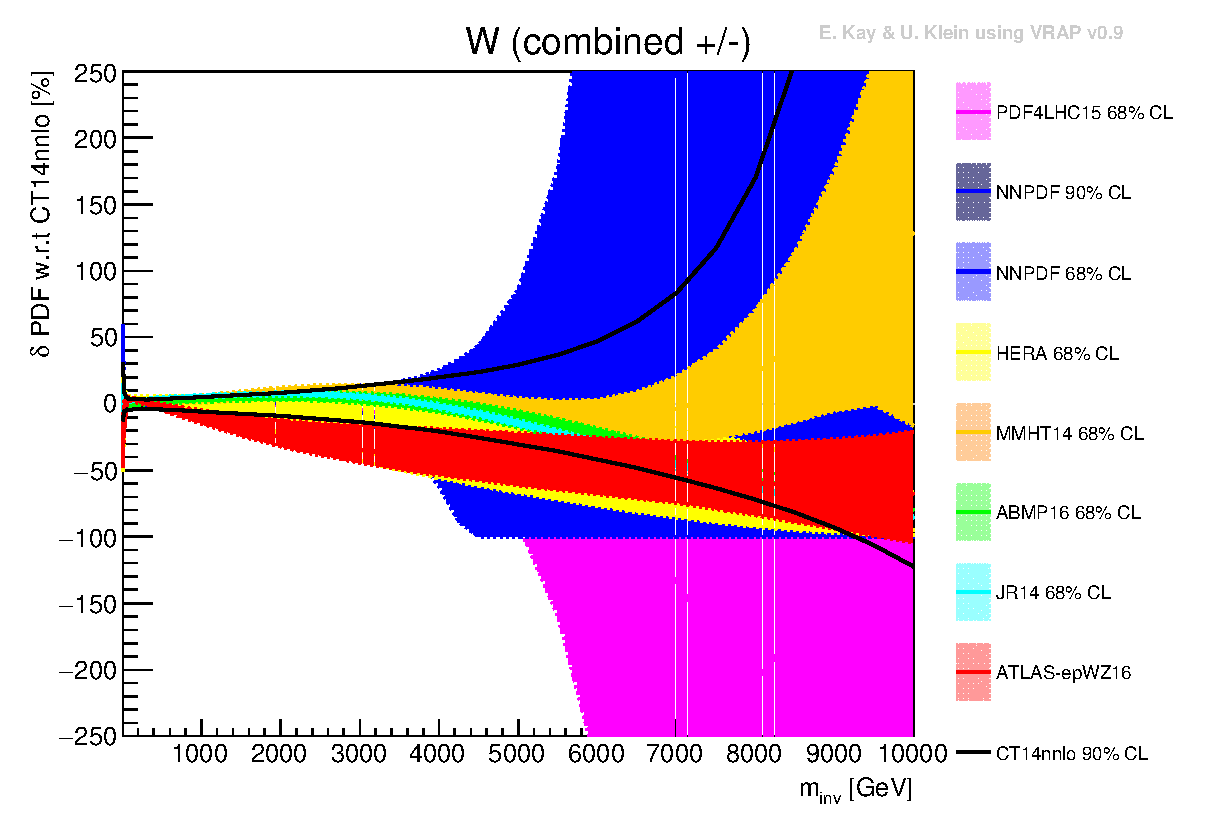
\includegraphics[width=.9\linewidth]{plots/PDFs/SUMMARY_ALLNEW/Wcomb.eps}
%
%	\cend
	\li{All fits for systematics are provided as functions which are used in LPXKfactorTool.}

	
\end{frame}


\begin{frame}
	\frametitle{NNLO QCD PDF Uncertainties}
	
	\vspace{15pt}
	
	\li {Full set of up/down/central NNLO cross section values has been produced for all modern NNLO PDF sets.}
	
	\li {Various prescriptions are required to calculate the upper and lower uncertainties associated with each PDF set.}
	%\lii { Hessian (asymmetric and symmetric prescriptions), treatment for MC replicas, mixture of Hessian treatment with extra variation uncertainties for HERA 2.0 and ATLASep-WZ16.}    

	\vspace{-20pt}
	\cleft{.5}
	\begin{center}
		\includegraphics[width=.9\linewidth]{plots/PDFs/SUMMARY_ALLNEW/Zgamma.eps}
	\end{center}
	
	\cright{.5}
	\begin{center}
		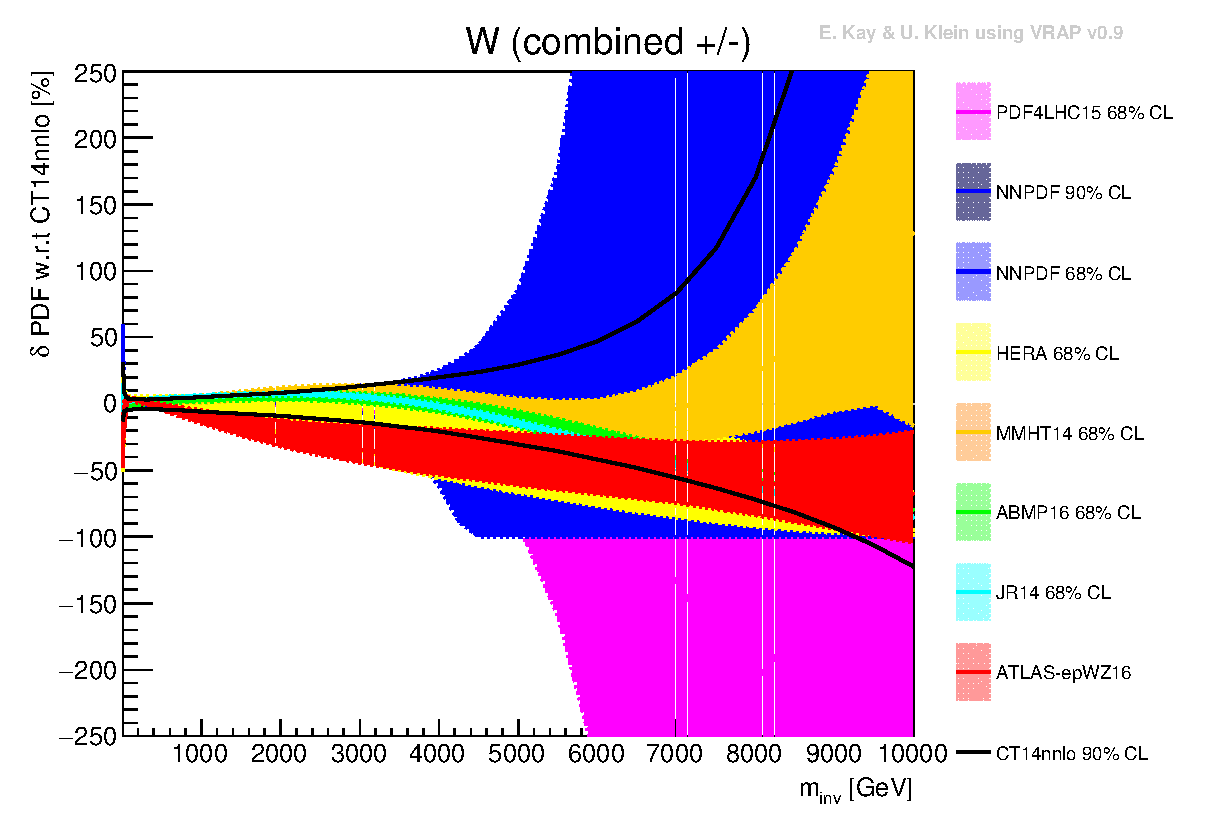
\includegraphics[width=.9\linewidth]{plots/PDFs/SUMMARY_ALLNEW/Wcomb.eps}
	\end{center}
	
	\cend
	{\scriptsize{
	Note: NNPDF(hence PDF4LHC) cross-sections become very small at high mass \& lead to negative predictions (see backup)}}
\end{frame}